\section{Security Model}

The BiobankCloud environment deploys strong security features for concerns such as confidentiality, integrity and non-repudiation ~\cite{BBCSEC} of data access. This includes authentication, authorization, and auditing. The system allows defining different roles with different access privileges. In designing the system, we applied the Cloud Privacy Threat Modeling~\cite {CPTM} approach to identify the privacy requirements of processing sensitive biomedical data.


Figure \ref{fig:security} shows the different components of the employed security mechanisms. All BioBankCloud services are protected behind the firewall and only accessible through the secure interfaces over HTTPS channels.


\begin{figure}[h]
\centering
\includegraphics[width=\textwidth]{./imgs/security.png}
% stack.eps: 0x0 pixel, 300dpi, 0.00x0.00 cm, bb=0 -1 805 312                                                                                                                                               
\caption{Security framework authorizes access to the BiobankCloud via the LIMS.}
\label{fig:security}
\end{figure}

\vspace{-5mm}

\subsection{2-Factor Authentication}
The authentication services map the person accessing the platform to a user identity. We provide 2-factor authentication using smart mobile devices or Yubikey \footnote {Yubikey Manual,http://www.yubico.com} hardware tokens to support different groups of users. Users send authentication requests via a Web browser to the authentication service that runs instances of the time-based one-time password (TOTP) and Yubikey one-time password (YOTP) protocols.

\vspace{-5mm}
\subsubsection {Mobile Authentication}
The mobile user supplies an one-time generated password by the Google Authenticator \footnote{Google Authenticator, https://code.google.com/p/google-authenticator/} in addition to a simple password that was decided during the account registration. The login page authenticates the user to to the platform using the TOTP module as an implementation of the RFC 6238 \footnote{Time-Based One-Time Password (TOTP), http://tools.ietf.org/html/rfc6238}.   

\vspace{-5mm}
\subsubsection {Yubikey Authentication}
The Yubikey user enters the Yubikey device into a USB port. The user enters the simple password that was decied during the account registration and pushes the Yubikey button. The Yubikey login page authenticates the user to the platform via the YOTP module.

\vspace{-2mm}
\subsection {Access Control}
The access control component ensures authorized access to genomics data as internal objects or different services within the platform. This is accomplished through a role-based access control (RBAC) model and authorization of data access on the HDFS, for example, a data owner adds/revokes members to a study and assigns privileges to access the study.
% 
% \subsubsection {Role-Based Access Control in HDFS}
The proposed RBAC model contains information about the roles of individuals within the organization and the associated levels of access to services.
\begin{itemize}
\item Administrator: group of users who acts as the platform manager and Ethics Board.
\item Auditor: group of users with access to audit trails for auditing.
\item Data Provider: group of users who create studies, upload data and assign members to studies.
\item Guest: general visitors to the platform who are able to request an account to use the services.
\item Researcher: users of the platform that can join a study to run workflows. Researchers also can become data providers through creating a new study and uploading data to the platform.
\end{itemize}

\vspace{-5mm}
\begin{figure}[h]
 \centering
 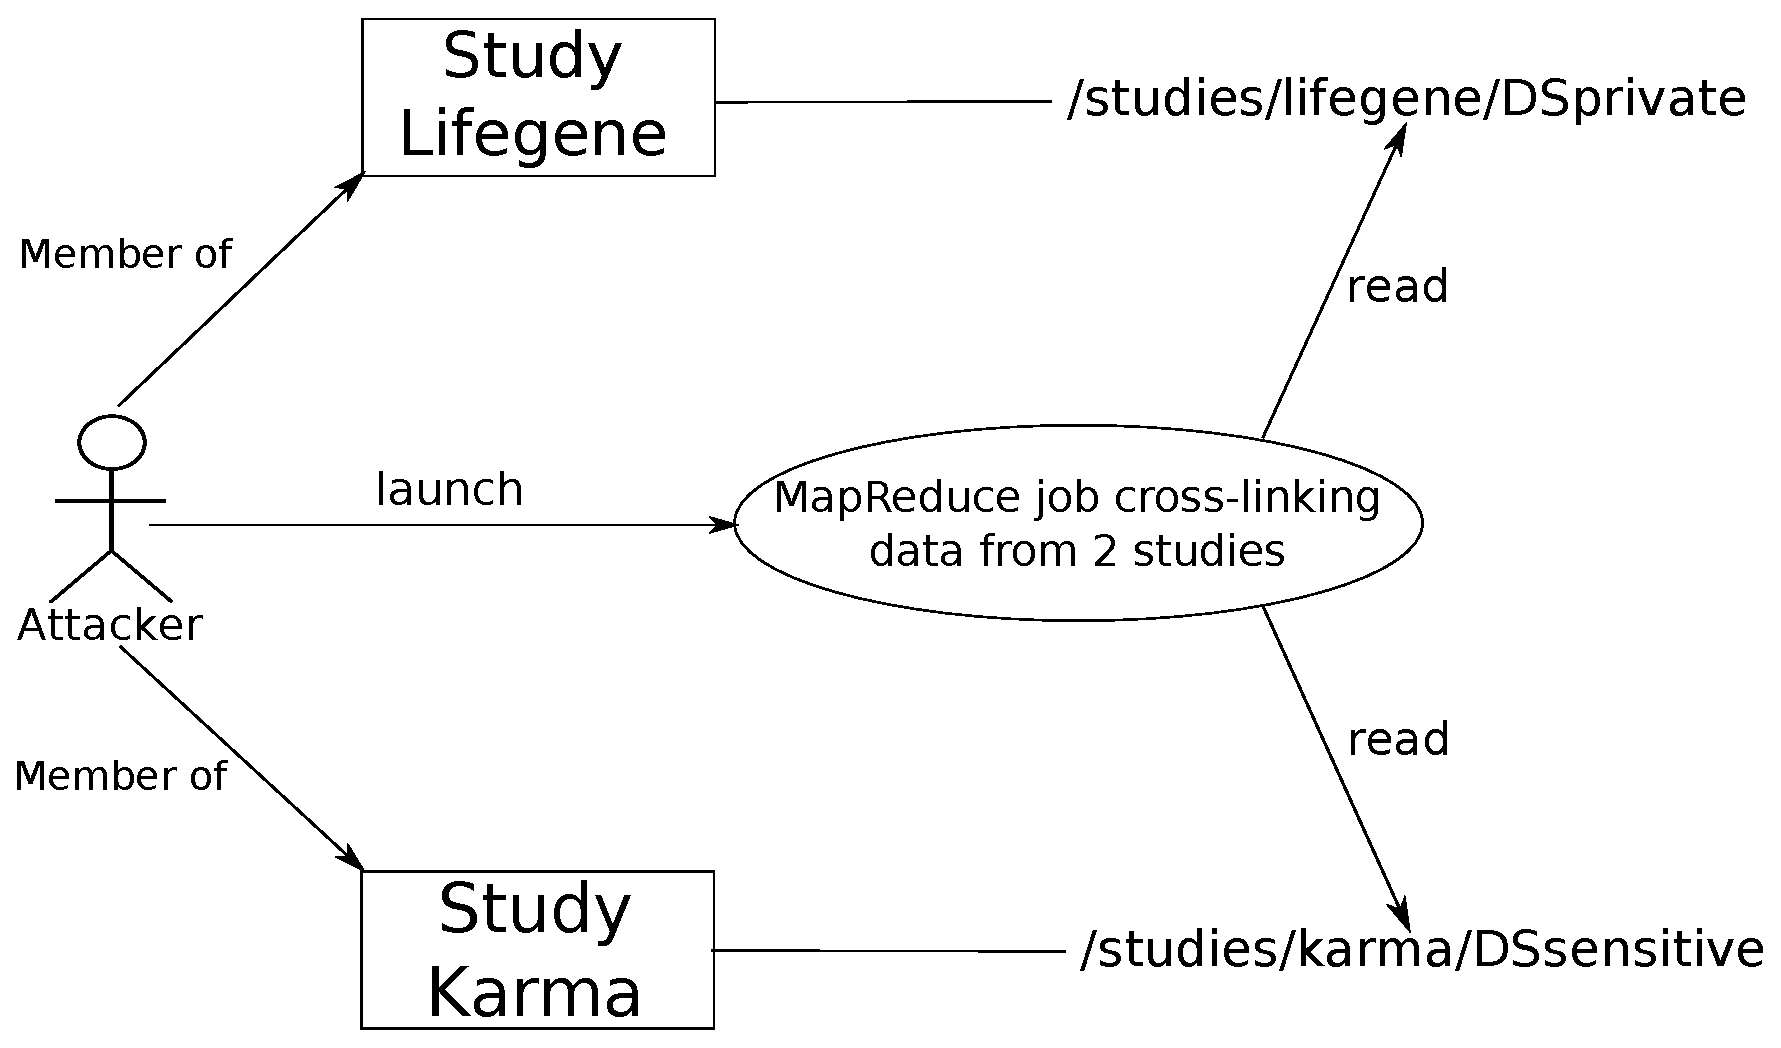
\includegraphics[scale=0.3]{./imgs/studyIsolation.eps}
 % studyIsolation.eps: 0x0 pixel, 300dpi, 0.00x0.00 cm, bb=0 -1 839 486
	\caption{Access control with the same HDFS user ID in both studies means that the attacker can cross-link data from both studies.}
	\label{fig:ac:problem:isolation}
\end{figure}
\vspace{-5mm}

A user may have different roles in different Studies. For example, be a Data Provider in one and a Researcher in another. For example, a user that creates a DataSet in a Study has the role of Data Provider and that user becomes the the owner of the folder and its files in HopsFS. However, that same user may be a Researcher in a different Study and not be allowed to create DataSets, but may read existing DataSets in the Study for the purpose of running analysis jobs. At the filesystem level, that user would be allowed read those DataSets by its user ID being a member of a group that has read privileges on the DataSet.

Now consider what an attacker with such privileges at the filesystem level can do. The attacker could write a program (like a MapReduce job) that cross-links data from DataSets in the different studies. In the filesystem, the DataSets are just files/directories with owner/group/world privileges, and the user is owner of one set of files and a member of a group with read privileges on another set of files. The problem here is that, if, at the filesystem level, we use the same user ID to represent the user in both Studies, then there is nothing preventing that user from writing a program that cross-links both DataSets, see \ref{fig:ac:problem:isolation}. Access control lists would not help solve this problem, although attribute-based policies could fix this - but they are not considered at the filesystem level due to their poor performance.

% Ultimately, the roles are enforced by owner, group, and world filesystem privileges in HopsFS. 

Our solution is to generate a new user ID for every member of every Study. The new user ID is a composite ID, consisting of both the user's global ID and the Study name. In addition to this, for every DataSet created, a new group is created, and all members of the Study where the DataSet was created that have an appropriate role are added to the new group. This method also enables us to safely share DataSets between studies. If a DataSet is shared with a different Study to the one where the DataSet was created, then the members of the different study with appropriate roles can be added to the group created for the DataSet. HopsFS can subsequently enforce these privileges using owener/group/world access rights, as programs that are run from within a Study are run with the study-specific ID. The only files in HopsFS that the study-specific ID will have privileges to access are DataSets from within that Study and DataSets that are shared with that Study. 
% With the study-specific user ID having either owner or group privileges on files in DataSets (depending on whether the user created the DataSet or not), HopsFS can now enforce the RBAC model using owner-group-world privileges.


% \begin{figure}[h]
%  \centering
%  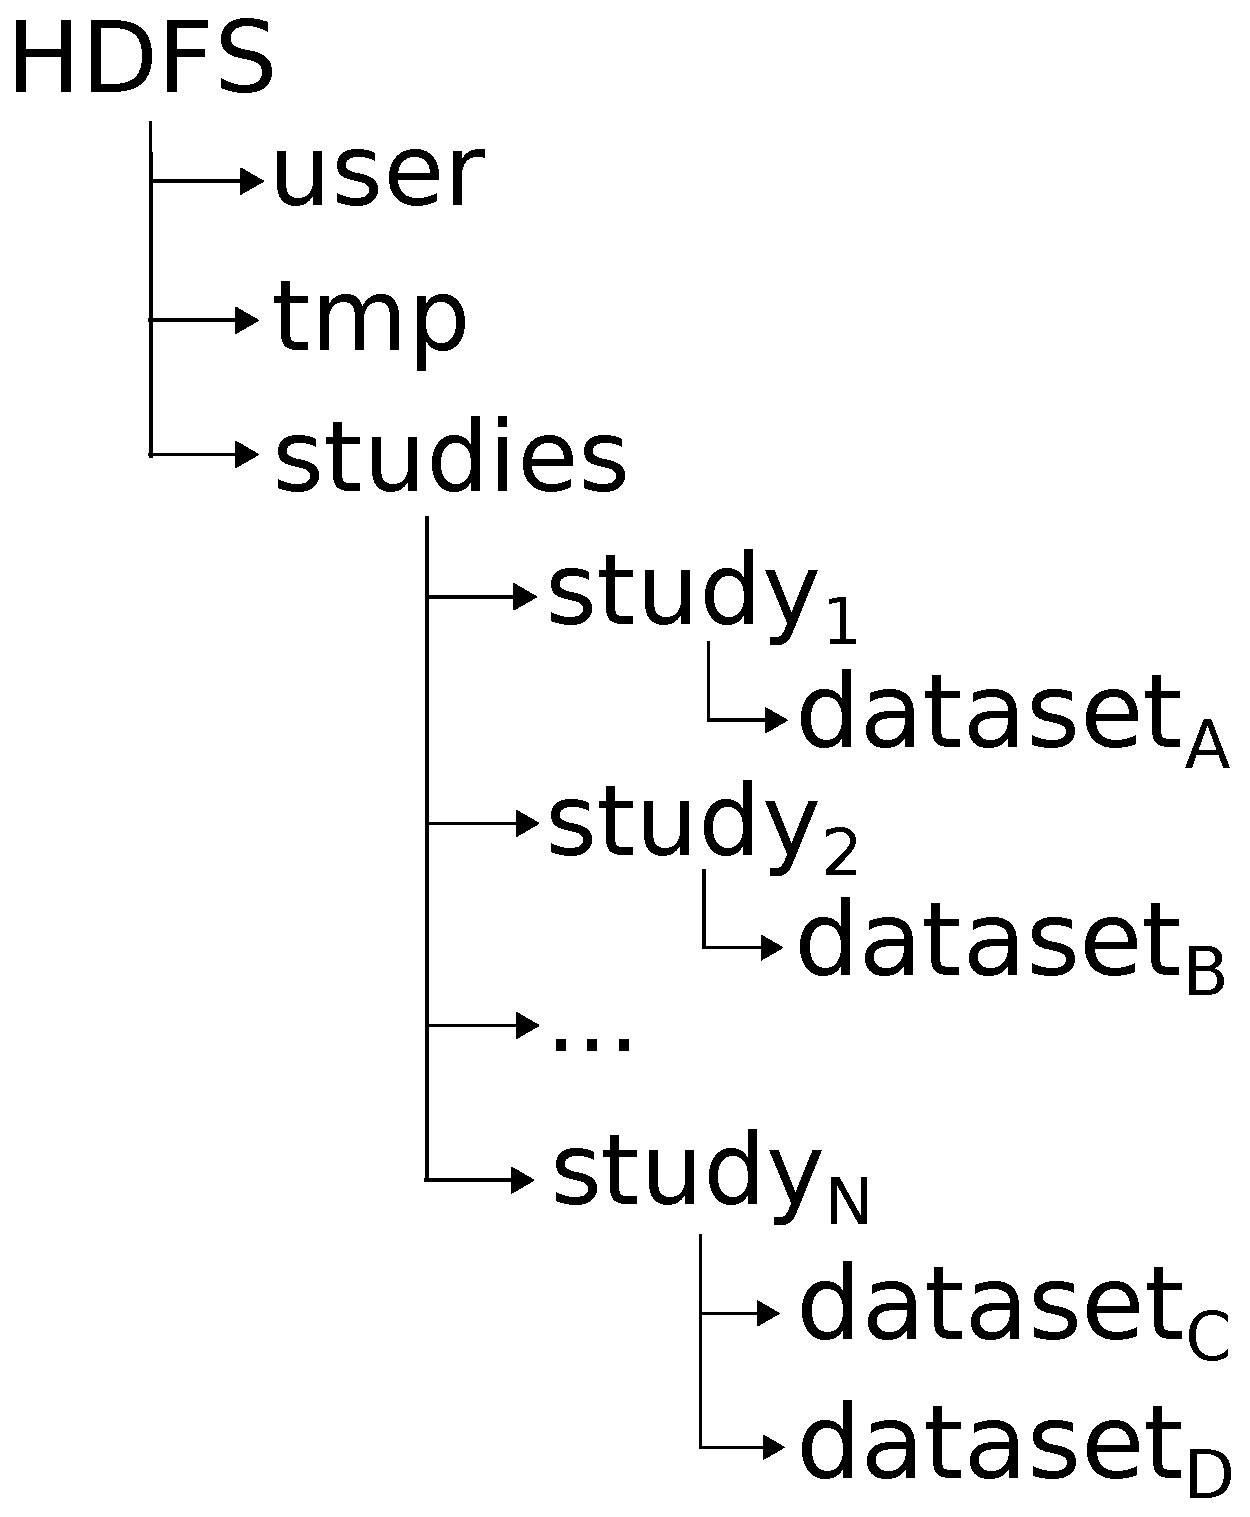
\includegraphics[scale=0.2]{./imgs/HDFS-structure.eps}
%  % HDFS-structure.eps: 0x0 pixel, 300dpi, 0.00x0.00 cm, bb=0 -1 584 711
%  \caption{Filesystem structure in HDFS containing Studies and DataSets.}
% \end{figure}


\subsection {Auditing Service}
Finally, the auditing service enables the platform administrator or an external auditor to discover the history of accessing the platform to detect any violation to a policy. It includes several contexts \
such as role, account, study, and login audits. The secure login service assures that actions that are taken by the users are registered for tracing and auditing purposes. Each log event contains informat\
ion such as initiator, target, IP/MAC addresses, timestamp, action, and outcome.
